\documentclass{book}
\usepackage[english]{babel}
\usepackage[utf8]{inputenc}
\usepackage{float}
\usepackage{graphicx}
\usepackage{subfig}
\usepackage{hyperref}
\usepackage{wrapfig}
\usepackage{listings}
\usepackage{fullpage}
\usepackage{caption}
\usepackage{cite}

\begin{document}

\begin{titlepage}
   \begin{center}
       \vspace*{1cm}

       \textbf{Electricity Bill Price Prediction}

       \vspace{0.5cm}
       Analysis based on European Union integration level
            
       \vspace{1.5cm}
       \textbf{Francesco Cabras}
       \vfill
       
\includegraphics[width=0.4\textwidth]{Images/unitn.png}            
       \vspace{0.8cm}
            
       Dipartimento di Matematica\\
       Università degli Studi di Trento\\
       Italy\\
       \today
            
   \end{center}
\end{titlepage}

\chapter*{Introduction}

Electricity bills are among the most important expenses for families around the world, at least for the lucky households that have access to it. In distinct countries the price of electricity of course is different, and it is not only always easy to acknowledge which are the reasons behind these gaps. One could think that the key factor is in the supply: how much it costs to actually source energy, getting electricity and especially distribute it among households. In recent years many countries around the world have gone through liberalization of their electricity markets: the result is that consumers can choose among different suppliers, and may decide to modify the profile of their demand to reduce their costs \cite{867149}. This means that the demand of electricity has become more elastic. Another trend that has gone through in recent years has been the increase in the renewable sources of energy. To measure the effect of such changes on the price of the good is the main aim of this document. The first idea is to have a look at the amount spent by households aroung the world for their electricity bills.  In \textit{Figure 1} the countries are colored on the basis of the price of electricity, measured in US dollars per kWh \footnote{World Bank data, 2020}.

\bigskip
\begin{figure}[H]
\begin{center}
\captionsetup{justification=centering}
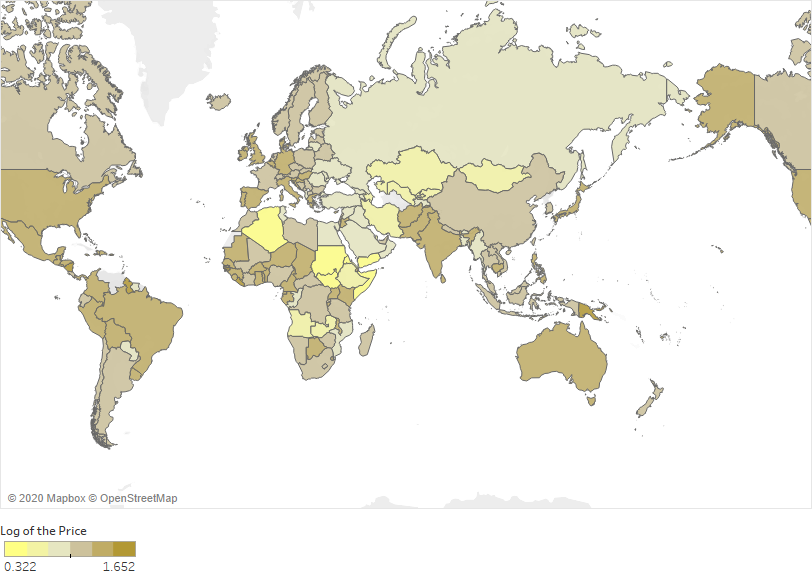
\includegraphics[width=0.7\textwidth]{Images/world2020.png}
\caption{The more expensive electricity is, the darker the color. }
\end{center}
\end{figure}
\bigskip

The more intense the red color, the more expensive electricity is. Interestingly, the country which appears as the most intensely red-colored is among the ones that has the easiest access to resources for getting electricity: \textbf{Venezuela}.The reason behind this finding is that in recent years this country has been suffering from exceptional inflation: the take-home message, however, is that the political and macro-economical frameworks are extremely important for the final price of this good.\\

Apart from South America, also in Africa some results are quite interesting: looking at the pale color of countries like South Sudan or Somalia, which are among the poorest in the world, the reader may think that to wealthier country consistently should correspond higher electricity price, given that there is no sky-high inflation. If however, for instance, bordering countries as Algeria and Niger countries are considered, this simple hypothesis does not work: the former has an electricity price of 2.1 dollars per kWh and a gdp per capita of 4,114.72 dollars. In the latter, instead, electricity price corresponds to 21.3 dollars per kWh (10 times with respect to Algeria) but the gdp is merely 413.98 dollars (almost one tenth with respect to Algeria). Since inflation is not really a problem in Niger, this is a hint that the link between economic development and electricity price is not that elementary. The particular problem with Niger is its extremely low electrification rate: only one in seven Nigeriens have access to modern electricity services, and just four percent of rural residents have access through the national utility. The country's total energy consumption per capita is 44 kWh of electricity. It is the second lowest energy consumption per capita in West Africa, behind Guinea Bissau, and the ninth lowest in the world. 

\subsection*{Access to Electricity}

While the whole share of Algeria inhabitants has access to the grid, this is not the case for Niger, where only part of the relatively wealthier urban population does. This explains why the price is not related with the gross domestic product per capita: since only the wealthy population can afford to have access to the grid, the prices can be kept higher. In this case a loop is entered, since prices are also high because network costs are shared among few people, and network costs are the most important component in the final electricity price paid by households. In \textit{Figure 2} it is showed how electricity price (in dollars per kWh) is related to population share having grid access, for countries with no universal electricity service.

\bigskip
\begin{figure}[H]
\begin{center}
\captionsetup{justification=centering}
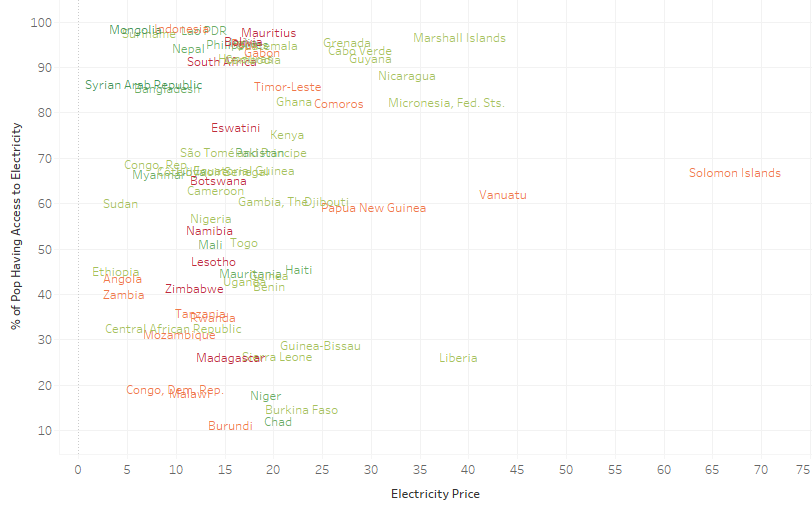
\includegraphics[width=0.9\textwidth]{Images/accessNAMES.png}
\caption{The more southern the country, the redder the color. }
\end{center}
\end{figure}
\bigskip

Although the countries providing little electricity access to its population also have low gross domestic product, prices are not that low with respect to wealthier and more electricity-intensive countries. In \textit{Figure 3} it is represented how countries with little grid access are concentrated in Africa: in recent years, Asian countries (especially India) have made important steps forward in this sense.

\bigskip
\begin{figure}[H]
\begin{center}
\captionsetup{justification=centering}
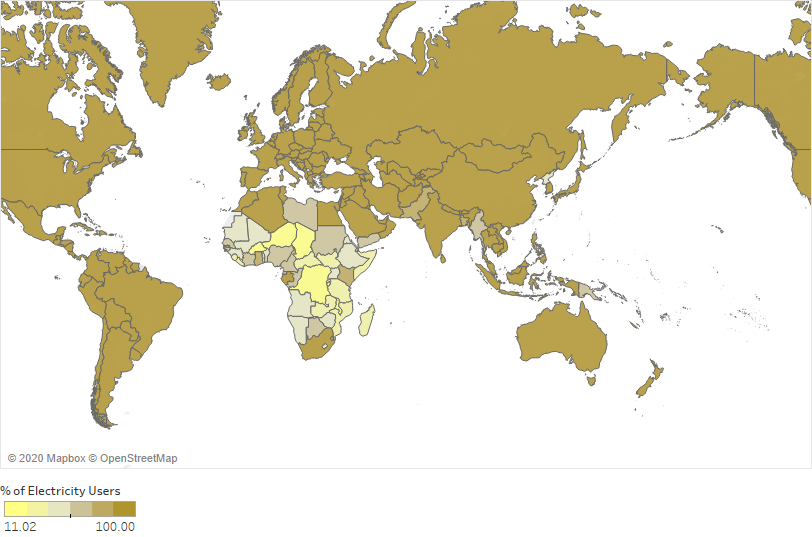
\includegraphics[width=0.7\textwidth]{Images/access.png}
\caption{Share of population having grid access. }
\end{center}
\end{figure}
\bigskip

\subsection*{Production}

Access to electricity is linked to production and consumption patterns inside a country. Electricity is not freely available in nature, so it must be "produced" (that is, transforming other forms of energy to electricity). Apart from a slight decrease during the 2008 crisis years, electricity production has been increasing constantly in recent years, with China having overcome United States as the main producer.\\

\textit{Table 1} illustrates which are the main electricity generators, with most recent data available. It is interesting to notice the leap of China which was able to increase its generation by five times of the amount it was producing in 2000, with an average increase of 5 percent per year. The United States also increased its production, but not at the pace of China. India was only the $7_{th}$ biggest producer in 2000, and also was able to climb the rankings quite fast in order to allow for its economy to grow. Japan, instead, saw its production decrease in the same time period.

\bigskip
\begin{table}[H]
\begin{center}
\begin{tabular}{|c|c|c|}
\hline
Country & Production (2000) & Production (2019)\\
\hline
China & 1,356 & 7,482\\
United States & 4,053 & 4,385\\
India & 570 & 1,614\\
Russia & 878 & 1,122\\
Japan & 1,068 & 1,013\\
Canada & 606 & 649\\
\hline
\end{tabular}
\caption{Major Electricity Producers (in KwH), Enerdata.}
\end{center}
\end{table}

If the focus shifts to European countries, Germany and France turn out being the two major producers in the continent, followed by the United Kingdom. European situation is illustrated in \textit{Figure 4}.

\bigskip
\begin{figure}[H]
\begin{center}
\captionsetup{justification=centering}
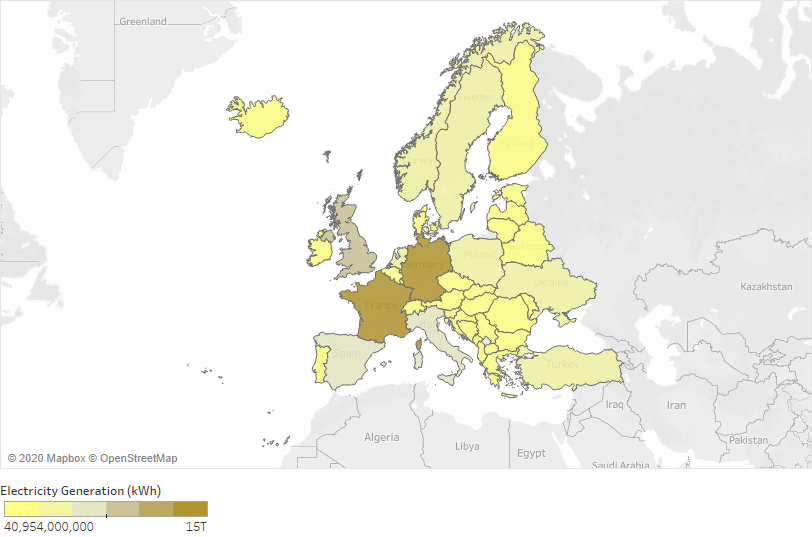
\includegraphics[width=0.7\textwidth]{Images/prod.png}
\caption{European countries and corresponding electricity generation capacity. }
\end{center}
\end{figure}
\bigskip

\subsection*{Distribution}

Of course producing electricity shall be a problem for certain countries, which lack the necessary resources. But an even more significant issue is often the absence of the necessary infrastructure to distribute this good. For poor regions in particular, electricity distribution losses represent  a big concern that hinder their economic development. \textit{Table 2} shows which are the countries that have the least efficient electricity distribution infrastructure.

\bigskip
\begin{table}[H]
\begin{center}
\begin{tabular}{|c|c|}
\hline
Country & Losses (\%)\\
\hline
Togo & 71\\
Libya & 69.7\\
Haiti & 60.1\\
Iraq & 50.6\\
Congo, Rep. & 44.5\\
Niger & 41.8\\
\hline
\end{tabular}
\caption{Distribution Losses (\% of output), World Bank data.}
\end{center}
\end{table}

Sadly, most of the distribution losses are associated with very poor countries, in which the access to electricity is limited. 

\subsection*{Consumption}

Since the major costs associated with electricity is actually the way of transporting it from one place to another, most of the electricity produced in one country actually remains inside that country until it is consumed. This explains why the major electricity producers are also the major electricity consumers. However, there are still marginal differences among these rankings. \textit{Table 2} shows which are the principal electricity consumers in the world.

\bigskip
\begin{table}[H]
\begin{center}
\begin{tabular}{|c|c|c|}
\hline
Country & Consumption (2000) & Consumption (2019)\\
\hline
China & 1,138 & 6,510\\
United States & 3,590 & 3,865\\
India & 376 & 1,230\\
Russia & 693 & 922\\
Japan & 986 & 918\\
South Korea & 263 & 553\\
\hline
\end{tabular}
\caption{Major Electricity Producers (in KwH), Enerdata.}
\end{center}
\end{table}

Also in this case, the behavior of Asiatic countries is the most interesting. China, India and South Korea have experience a major boost in their electricity consumption while Japan decreased its value in the last 20 years. China is the country which consumes (and produces) the largest share of electricity because it is also the most populated. Data regarding consumption per capita represented in \textit{Table 3} can result be even more interesting.

\bigskip
\begin{table}[H]
\begin{center}
\begin{tabular}{|c|c|c|}
\hline
Country & kWh consumption per Capita\\
\hline
Iceland & 53,832\\
Norway & 23,000\\
Bahrain & 19,597\\
Kuwait & 15,591\\
Canada & 15,588\\
Finland & 15,520\\
\hline
\end{tabular}
\caption{Countries with highest consumption per capita values, World Bank data.}
\end{center}
\end{table}

There are certain countries that are particularly ill-suited for the existence of individuals, and a large amount of energy has to be consumed in order to improve their well-being. It is the case of Iceland and Norway, where temperatures are very low and during winter months sunlight is available only for few hours. Or it is the case of Bahrain or Kuwait where contrarily it is simply too hot.

\textit{Figure 5} also shows how European countries with highest consumption per capita are located in the North, where temperatures are lowest.

\bigskip
\begin{figure}[H]
\begin{center}
\captionsetup{justification=centering}
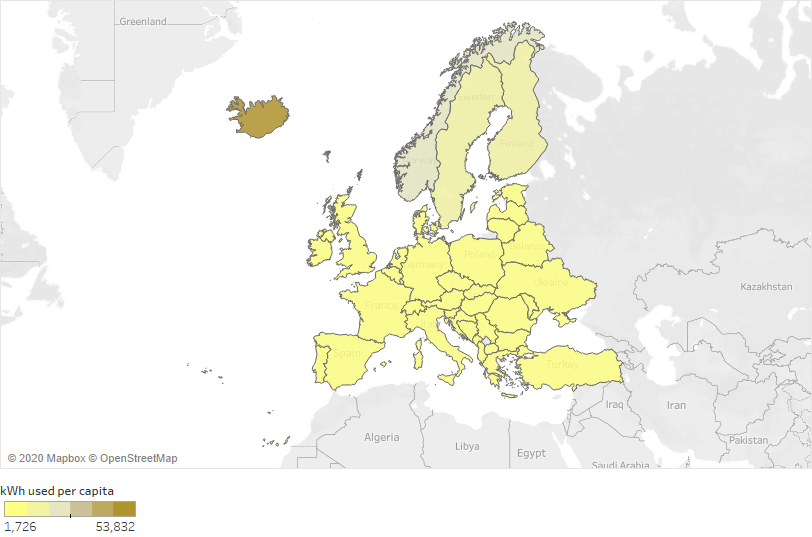
\includegraphics[width=0.7\textwidth]{Images/cons.png}
\caption{European countries and corresponding consumption per capita values, World Bank data. }
\end{center}
\end{figure}
\bigskip

\section*{European Union Electricity Market}

Electricity is not an easily tradable product, as it needs hundreds of  legal rules and technical standards to be agreed upon before it can become freely marketable. Electric power is, after all, not more than a flow of electrons inside metallic wires of a massive, interconnected network. That is the reason why, for decades, electricity was considered to be an "anti-market" product, best suited to non-competitive markets like natural monopolies. \cite{glachant2014eu} Furthermore, the particular characteristics of electricity, such as non-storability and the continuous balance between demand and supply, supported the State intervention. The fact that this market is inclined to be a monopoly resulted in efficiencies, where State subsidies have been the rule to maintain a stable industry. \cite{domanico2007concentration} Nevertheless, there is one region in the world that has tried to overcome these "anti-market" barriers to create an extremely vast electricity market. That region is identifiable as the European Union. \\

The European Union because is a unique case of a large extended market in which member countries can exchange goods.  Liberalization of the economic markets and convergence are two of the main objectives in the Union. In particular, European electricity market liberalization represents the world's most large-scale cross-jurisdiction reform of the electricity sector involving integration of national markets. To reach such a big achievement took several years of time, and there are specific reasons why this process took so long:

\begin{itemize}

\item The objective of this project is to open up national monopolies’ market spaces to foreigners, which of course is a radical
project that inevitably leaves some parties unsatisfied.  One of the risks of market concentration is that big incumbents try to build
barriers in order to maintain their position and to foreclose the entrance of more efficient market actors. \cite{ringel2003liberalising}

\item In the last 25 years there has been no wave of disruptive technological innovation to challenge the incumbent energy
giants.

\item the national arrangements that had been developed between industry players and public authorities could not be easily merged at the EU level into a common scheme.
\end{itemize}

Creating a market that is actually free, however, is not an easy matter, and that's why there are still wide differences in the amounts households from different member countries pay for electricity. Although the pace of the liberalization is steady, the integrated European electricity market is yet to be achieved. \\

\subsection*{Taxation}

Taxes account for a sizable share of the final prices consumers pay for energy around the EU and can have a strong impact on consumption patterns, the type of energy consumed and their use. There is disagreement among European countries for much households should pay in their bills, and the consequence is wide differences in tax rates. Belgium, Ireland, Germany and Denmark are the member states where electricity is the most expensive. However, these four countries present different tax rates: Belgium and Ireland citizens pay a high price because electricity is actually expensive excluding taxes and levies while Germany and especially Denmark pay such a high price precisely because of taxes and levies. This behavior is well represented with \textit{Figure 2}, where household electricity prices are plot both including and excluding taxes and levies. Prices are lowest in Bulgaria and Hungary, whose inhabitants pay one third of the amounts Danish citizens pay in their bills. 

\bigskip
\begin{figure}[H]
\begin{center}
\captionsetup{justification=centering}
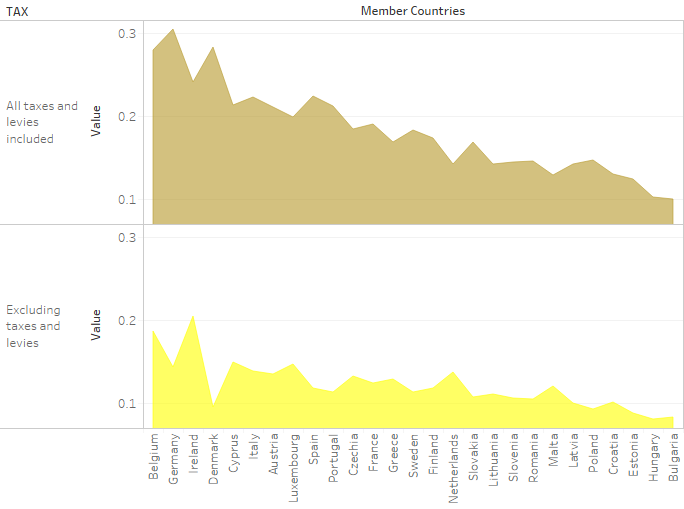
\includegraphics[width=0.7\textwidth]{Images/Taxes.png}
\caption{2019 (second semester) data, electricity prices. }
\end{center}
\end{figure}
\bigskip

The average final price paid by European households is 21.7 cents per KwH including taxes and 12.8 cents per KwH excluding taxes, which make up an average of around 6 cents of taxes per KwH. Over time, also taxes tend to change: in the second semester of 2007 the price paid by European households fell with respect to the first semester by 3 cents, while the the electricity price itself decreased only by a cent. This means that most of the drop was due to a decrease in taxes. \textit{Figure 3} shows how electricity prices for European citizens changed over time, on average.

\bigskip
\begin{figure}[H]
\begin{center}
\captionsetup{justification=centering}
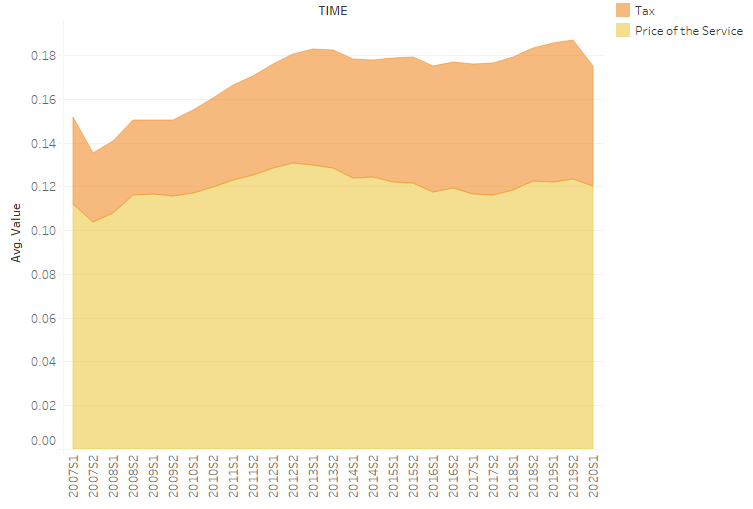
\includegraphics[width=0.7\textwidth]{Images/TaxesTime.png}
\caption{2019 (second semester) data, electricity prices. }
\end{center}
\end{figure}
\bigskip

\subsection*{Inflation}

As all other commodities, the price of electricity tends to increase over time at a similar pace with respect to inflation. The average increase in prices in a given country is an obvious cause for electricity price surge. The levels of inflation are over time converging, as it should be for such a tied market, and the pace of such convergence became even more steady after the global financial crisis. \cite{brovz2018dynamics} The body which is charge for controlling the inflation level in the Euro area is the European Central Bank, and the primary objective of its monetary policy is to maintain price stability. The ECB aims at inflation rates of below, but close to, 2\% over the medium term. The ECB failed to keep inflation under this level for the first years of the 21th century, before the 2008 financial crisis, but after this the inflation level dropped and never got back to such high levels. Such inflation target was highly debated in recent times, especially after the Federal Reserve has relaxed the same 2\% target.\\

As it is possible to discern from \textit{Figure 4}, the inflation level and the electricity price tend to show a similar trend. The average level of prices in 2015 is used as a benchmark and is denoted by a 100 in the plot. Interestingly, however, the electricity price has had its peak in 2012, while inflation continued being positive until now. 

\bigskip
\begin{figure}[H]
\begin{center}
\captionsetup{justification=centering}
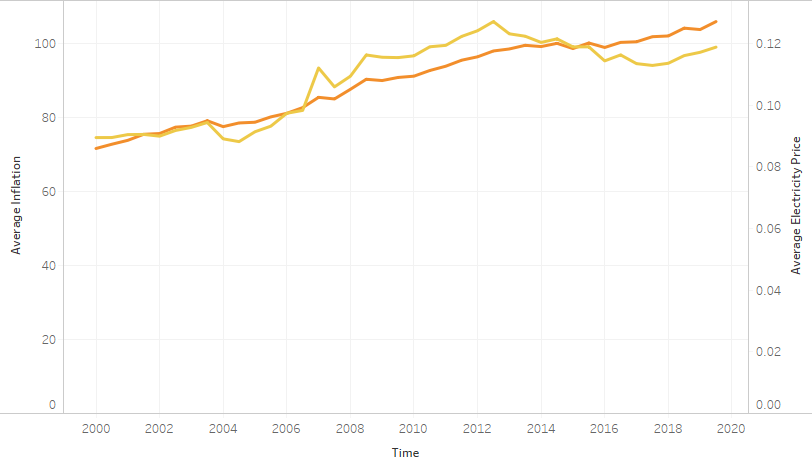
\includegraphics[width=0.8\textwidth]{Images/inf.png}
\caption{Price of electricity and inflation level in the European Union . }
\end{center}
\end{figure}
\bigskip

The behavior of inflation depends both on structural and on short-term factors. The inflation rate over long periods is determined by the extent to which the rate of money growth (which is controlled by the ECB or by national central banks in non-euro countries) exceeds the growth rate of real output. Short-run fluctuations are instead due to demand shocks, e.g. sizable increases in government spending, and supply shocks, e.g. sharp rises in the oil price. \cite{ball1993causes}

\subsection*{Market Concentration}

The directive 2003/54/EC requires that all non-household customers can freely choose their electricity by 1 July 2004, with successive full market opening including all household customers within three years. Most of the European Union electricity market is now at least formally, open to competition; this was not the case a few decades ago. However, most national electricity market are still dominated by relatively few companies and small consumers seem quite resistant to switching supplier. \cite{jamasb2005electricity} \\

The European Union is fighting monopolies in the electricity sector for the simple reason that the market price is supposed to be higher with respect to a situation of competition. In the 1990s the United Kingdom was the front-runner of electricity reforms, while France has often been regarded as a country averse to moving away from public monopoly. \cite{fiorio2009reform} In \textit{Figure 9} European countries are colored according to their level of market concentration. It is possible to notice how, most notably, the market concentration levels are quite heterogeneous among countries, with France, Estonia and Croatia experiencing very different levels with respect to United Kingdom, Poland and Spain. 

\bigskip
\begin{figure}[H]
\begin{center}
\captionsetup{justification=centering}
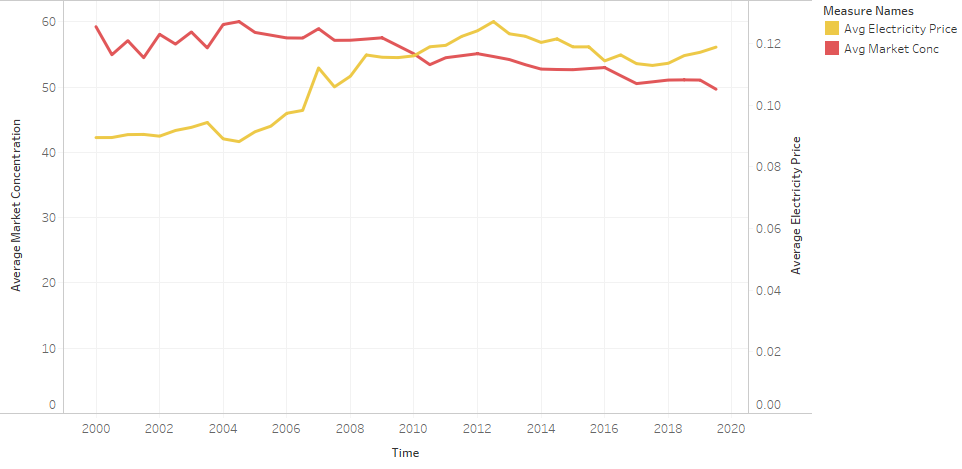
\includegraphics[width=0.6\textwidth]{Images/conc.png}
\caption{Market Share of Largest Producers for European countries, 2018 data. }
\end{center}
\end{figure}
\bigskip

In any case, \textit{Figure 9} also demonstrates how, although the liberalization process has led to the disintegration of national monopolies, it did not lead to a disruptive fall in concentration within the sector. With an average value of the biggest  supplier market share of 50\% the European situation is quite far from the internal market and open competition. There still exist different national and regional markets with the presence of incumbents as main actors in each electricity market. Despite liberalization, the level of concentration is hence quite high.  In \textit{Figure 3}, the focus is on the biggest European markets over the last 20 years: Germany, Spain, France and Italy. It is interesting how notice how they all experienced a slight decrease in market concentration, but with France starting from a concentration value that stands out with respect to the others, with the most important supplier having a market share of 90\%.

\bigskip
\begin{figure}[H]
\begin{center}
\captionsetup{justification=centering}
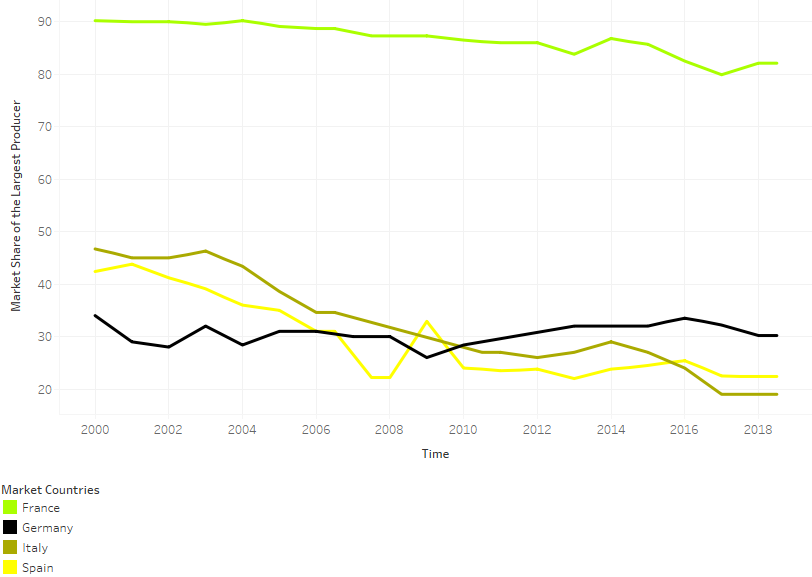
\includegraphics[width=0.6\textwidth]{Images/conc-mc.png}
\caption{Largest supplier market share for Germany, Spain, France and Italy over time. }
\end{center}
\end{figure}
\bigskip

One final note of caution: in this section the market share of the biggest supplier in the market was used as a proxy for market liberalization. The higher the share, the more the market is concentrated. However, looking at the largest supplier is a bit limiting and it is used only because data are available from Eurostat. A market in which only two suppliers share the whole market is completely different from one in which the biggest supplier controls half of the market and the rest of it is controlled by very little providers. Yet, the largest supplier market share variable value would be the same.

\subsection*{Gross Domestic Product}

The wealth and the productive capacity of a country are closely related to the consumption patterns of its citizens. Economic development stimulates greater demand for electricity in the long-run: the gross domestic product has an effect primarily on the quantity of electricity consumed. \cite{jamil2010relationship} Whether there is an effect not only on the quantity used but also on the price of the good is a more debated topic: \cite{lean2010multivariate} employs annual data for Malaysia from 1970 to 2008 to examine this causal relationship but found that there is no causal relationship between prices and economic growth. \textit{Figure 11} shows differences in GDP per capita, in US dollars. \footnote{World Bank data}

\bigskip
\begin{figure}[H]
\begin{center}
\captionsetup{justification=centering}
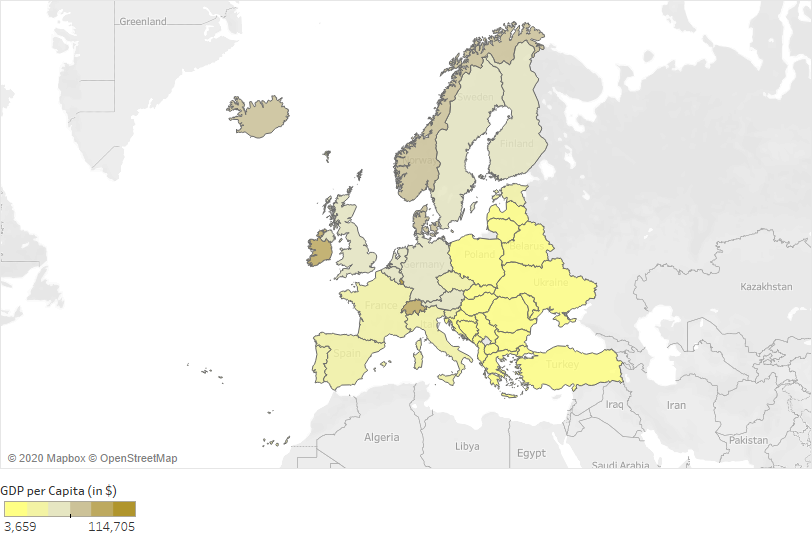
\includegraphics[width=0.6\textwidth]{Images/gdp.png}
\caption{Gross Domestic Product per capita for European countries (in Dollars). }
\end{center}
\end{figure}
\bigskip

Belgium, Ireland, Germany and Denmark are the European member countries for which electricity is the most expensive, and also corresponds to high GDP areas. In the last 20 years GDP tended to increase for European countries, even if the economic crisis incurred in the end of the first decade slowed down the growth process. Also the electricity price has tended to increase, although at different paces and more irregularly with respect to the Gross Domestic Product.\\

\textit{Figure 12} shows the behavior of real GDP per capita and electricity price (taxes excluded) for France and Germany, the two major economies in the European Union.  In this case inflation has been taken into account and in fact the absolute GDP values are not comparable with \textit{Figure 11}. Electricity is cheaper in France with respect to Germany by quite a significant amount, and Gross Domestic Product is also lower. For both countries there have been increase in the values of the two parameters, although with considerable less regularity when it comes to electricity price.

\bigskip
\begin{figure}[H]
\begin{center}
\captionsetup{justification=centering}
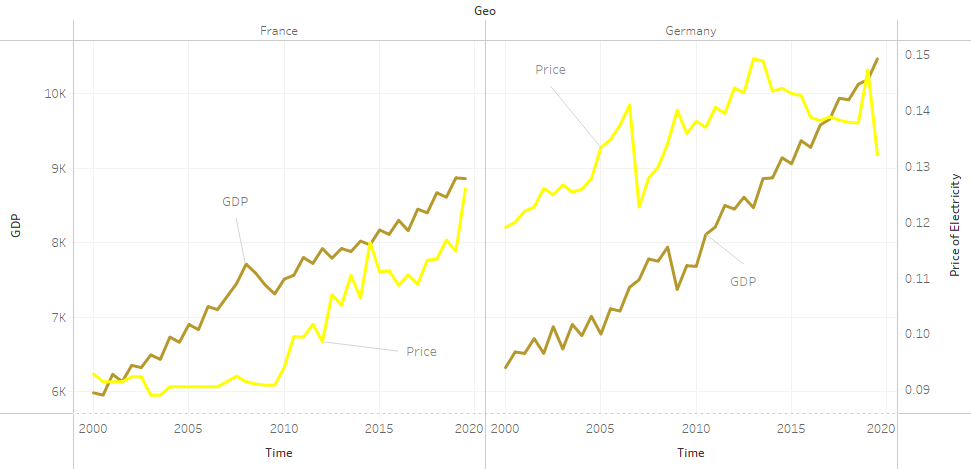
\includegraphics[width=0.8\textwidth]{Images/pri-gdp.png}
\caption{GDP per capita and Electricity Price over time for France and Germany. }
\end{center}
\end{figure}
\bigskip

\subsection*{Emission Intensity}

Depending on how it is produced, electricity can be associated with environmental degradation. A debated question in recent times is whether cleaner energy results in higher prices or rather the opposite. The \textit{Emissions Intensity} indicator is calculated as the ratio between energy-related GHG emissions and gross inland consumption of energy. It expresses how many tonnes CO2 equivalents of energy-related GHGs are being emitted in a certain economy per unit of energy that is being consumed.\\

All European countries successfully managed to decrease their emission intensity in the last 20 years, but with wide differences. Eastern countries which base their economy on energy production and distribution such as Ukraine and Georgia saw their emission intensity levels drop by one tenth in one year. Such result is mostly due to the very low levels of efficiency these countries were experiencing in the beginning of the century. In \textit{Table 4} emission intensity for most virtuous countries is summarized: the relative level in the table is benchmarked over the emission intensity level the country experienced in 2000 (i.e. level in 2000 = 100).

\bigskip
\begin{table}[H]
\begin{center}
\begin{tabular}{|c|c|}
\hline
Country & Emission Intensity \\
\hline
Ukraine & 90.9\\
Malta & 90.9\\
Georgia & 90.9\\
Kosovo & 91.3\\
Moldova & 91.3\\
\hline
\end{tabular}
\caption{Countries which reduced their emission intensity the most in the last 20 years.}
\end{center}
\end{table}

With \textit{Table 5}, instead, a summary is provided the countries which experienced the smallest drop in emission intensity in the last 20 years. It can be not that easy to match economic development with climate action, and progress in one field can hinder progress in the other.

\bigskip
\begin{table}[H]
\begin{center}
\begin{tabular}{|c|c|}
\hline
Country & Emission Intensity \\
\hline
Bulgaria & 97\\
Lithuania & 95.6\\
Luxembourg & 95.3\\
Cyprus & 95.2\\
Estonia & 95\\
\hline
\end{tabular}
\caption{Countries which reduced their emission intensity the most in the last 20 years.}
\end{center}
\end{table}

Eurostat does not provide absolute values for the Emission Intensity indicator, but the World Bank provides data for $CO_{2}$ emissions per capita. \textit{Figure 13} is helps to visualize which are the countries and most and least $CO_{2}$ intensive. One interesting area of focus for further discussion is the Baltic. To demonstrate how political decisions can result in building two radically different economies also for countries which are neighboring and similar, it is interesting to notice how Lithuania is one of the least polluting country in Europe and Estonia is instead the one that is polluting the most.

\bigskip
\begin{figure}[H]
\begin{center}
\captionsetup{justification=centering}
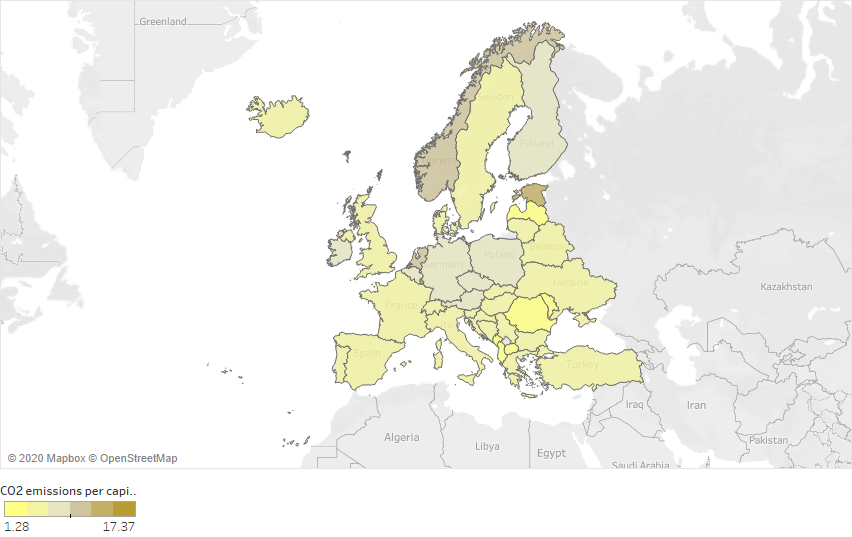
\includegraphics[width=0.7\textwidth]{Images/intensiti.png}
\caption{CO2 emissions (metric tons per capita). }
\end{center}
\end{figure}
\bigskip

\subsection*{Energy Mix}

The importance of energy on greenhouse gases emissions is reflected by the fact that 65\% of emissions in the World are currently due to the use and production of energy. This percentage rises up to 80\% in the European Union.\cite{marrero2010greenhouse} Energy production techniques and consequent polluting emissions vary greatly from one country or region to the next and can change significantly depending on the period. The term \textit{energy mix} refers to the combination of the various primary energy sources used to meet energy needs in a given geographic region. Variables at stake for the final choice of the energy mix include:

\begin{itemize}

\item The availability of resources domestically or the possibility of importing them;
\item The demand of energy which needs to be met;
\item Policy choices determined by political, economic, environmental and geopolitical factors.

\end{itemize}

Low income, developing countries tend to rely heavily on biomass energy and coal. \cite{international2009energy} As countries become wealthier, new technologies enter the market, and they substitute towards higher quality energy sources. \cite{csereklyei2016energy}

\subsubsection*{Coal}

Although the EU electricity system has modernised and become greener, it has also maintained its oldest and most polluting component: coal. As mentioned above, it is usually under-developed countries that rely heavily on coal. However, political decisions are also key in this sense. Poland has seen its economy grow in recent years, but still relies on coal heavily for electricity production. European countries which rely on coal the most are listed in \textit{Table 6}.

\bigskip
\begin{table}[H]
\begin{center}
\begin{tabular}{|c|c|c|}
\hline
\multicolumn{3}{|c|}{Electricity Prod. from Coal (\% of total)}\\
\hline
Country & 2015 & 2000 \\
\hline
Kosovo & 97.5 & 97.6\\
Poland & 80.91 & 96.3 \\
Serbia & 72.4 & 62.8 \\
Bosnia & 63.4 & 50.7\\
North Macedonia & 58.4 & 76.5\\
\hline
\end{tabular}
\caption{Countries which rely on coal sources for electricity generation the most.}
\end{center}
\end{table}

The trend toward reducing the impact of coal in the energy mix has been set in all corners of Europe, now the focus is on the timing. Even Germany, a country which is very careful on environmental matters, in 2015 still relied on coal for 44\% of its energy production. The share of fossil fuel in the EU electricity generation mix stands at 25 percent, having declined by only 5 percentage points between 2000 and 2015. This is a problem, since as \cite{tagliapietra2017beyond} points out, to generate the same amount of electricity, a coal-fired power plant emits 40 percent more CO2 than a gas-fired power plant and 20 percent more than an oil-fired power plant.

\bigskip
\begin{figure}[H]
\begin{center}
\captionsetup{justification=centering}
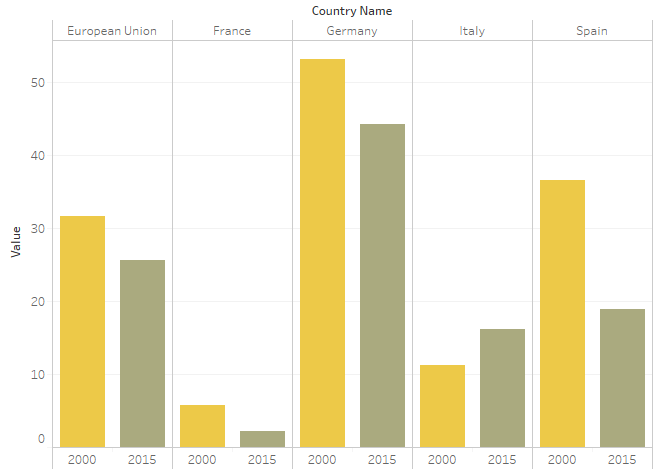
\includegraphics[width=0.5\textwidth]{Images/coal.png}
\caption{Electricity Production from Coal (\% of total). }
\end{center}
\end{figure}
\bigskip

\subsubsection*{Oil}

One traditional way of producing electricity is by fuel combustion: the raw material, oil, sits in deep underground reservoirs. Since the ultimate amount of oil is finite - and cannot be replenished once it is extracted and burned - it is not a renewable resource. Burning oil to generate electricity produces significant air pollutants, and this may also explain why this energy source is going out of fashion: in the 70s oil combustion was one of the main techniques for electricity generation, accounting for about one fifth of the total. After this, however, such share shrank constantly: in 2015 only less than 4\% of electricity is generated by fuel combustion. \textit{Figure 15} shows the trend in electricity generation from fuel combustion.

\bigskip
\begin{figure}[H]
\begin{center}
\captionsetup{justification=centering}
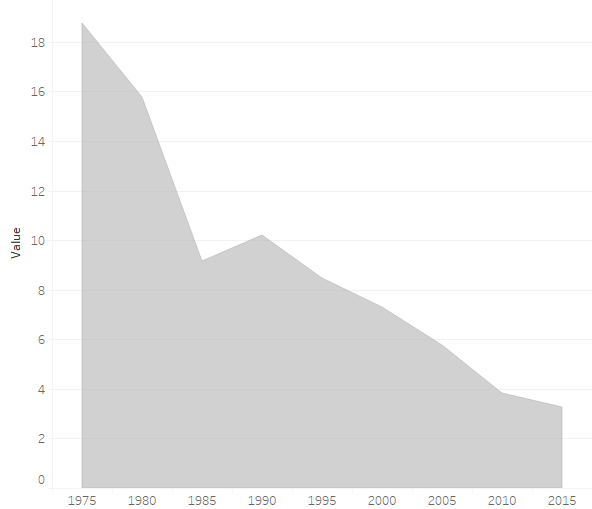
\includegraphics[width=0.5\textwidth]{Images/oil.png}
\caption{Electricity Production from Oil (\% of total). }
\end{center}
\end{figure}
\bigskip
 
Since oil can be used for producing electricity, one could easily infer that the price of the former could have an effect on the price of the latter. Oil price has showed significant fluctuations in the last 20 years. From 1999 until mid 2008 the price of oil rose significant thanks to the rising oil demand in Asian countries. The 2007-2008 financial crisis corresponded to a drop in the price of crude oil, followed by a fast recovery in the years after. The world price of oil was above 125 US dollars per barrel in 2012, and remained relatively strong above \$100 until September 2014, after which it entered a sharp downward spiral, falling below \$30 by January 2016. What happened is the so-called \textit{oil glut}, a serious surplus of crude oil that started in 2014 and accelerated in the next two years, with multiple causes. They include general oversupply as United States and Canadian oil production (obtained by fracking) reached critical volumes, geopolitical rivalries among oil-producing countries, falling demand across markets due to the slow down of the Chinese economy, and possible restraint of long-term demand due to environmental concerns. \textit{Figure 16} represents graphically what happened in the last 20 years, with all the up and downs the price of oil experienced.

\bigskip
\begin{figure}[H]
\begin{center}
\captionsetup{justification=centering}
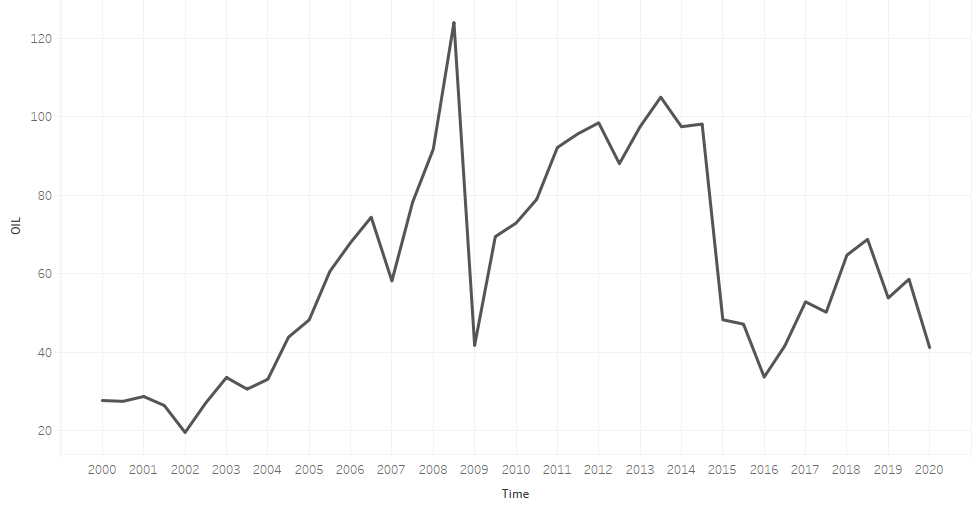
\includegraphics[width=0.6\textwidth]{Images/oilbeh.png}
\caption{Electricity Production from Oil (\% of total). }
\end{center}
\end{figure}
\bigskip

\subsubsection*{Nuclear Power}

Electricity can also be produced by a process which makes use of nuclear reactions. This type of energy has one of the lowest levels of fatalities per unit of energy generated compared to other energy sources, given that electricity generation by coal and oil combustion result in air pollution. \cite{markandya2007electricity} However, nuclear power is going out of fashion mostly because of Chernobyl and Fukushima disasters, which questioned its use in Europe. Germany was one of the most radical governments to abandon its nuclear energy program, having the greatest number of permanently closed nuclear plants among the 27 European Union member countries. In fact, it plans to shut down all remaining nuclear reactors by 2022. Having taken opposite political decisions, France still relies heavily on nuclear power generation. It has the second highest number of operable nuclear reactors worldwide and it is supposed to build an additional nuclear reactor. Leaving out France, most of the other European countries are going in the direction of a reduction in the share of energy produced by nuclear reaction. Only Slovakia is greatly investing in broadening its nuclear energy program, looking to add two further reactors to the four already in use. \textit{Table 7} summarizes the trend in nuclear energy production: the share of energy produced by reactors as percentage of the total in 2000 and 2015 is displayed.

\bigskip
\begin{table}[H]
\begin{center}
\begin{tabular}{|c|c|c|}
\hline
\multicolumn{3}{|c|}{Nuclear Energy (\% of total)}\\
\hline
Country & 2015 & 2000 \\
\hline
France & 77.6 & 77.6 \\
Slovakia & 56.9 & 53.6 \\
Hungary & 52.2 & 40.3 \\
Slovenia & 38.1 & 35 \\
Belgium & 37.5 & 58.1\\
\hline
\end{tabular}
\caption{Countries which rely on nuclear reactors for electricity generation the most.}
\end{center}
\end{table}

\subsubsection*{Renewable Sources}

The use of renewable energy for producing electricity has several potential benefits, including a reduction in greenhouse gas emission and a reduced dependency on fossil fuel markets (in particular, oil and gas). Additionally, it is considered safer with respect to nuclear production, due to the disasters experienced in the last 40 years. The increase in the share of electricity produced through renewable sources has been steady in the last 20 years, going from a share of 9.6\% of the total in 2004 to 18.9\% in 2004. While the EU as a whole is on course to meet its 2020 targets, some member states will need to make additional efforts to meet their obligations.
\textit{Figure 17} shows where each country is in the path towards more sustainable energy sources.

\bigskip
\begin{figure}[H]
\begin{center}
\captionsetup{justification=centering}
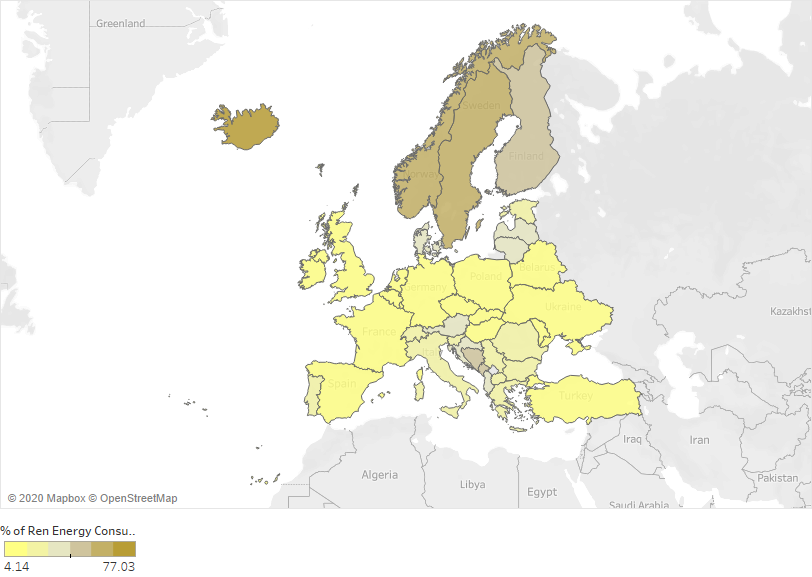
\includegraphics[width=0.7\textwidth]{Images/ren.png}
\caption{Renewable Energy Consumed (\% of total). }
\end{center}
\end{figure}
\bigskip

Northern countries have invested significantly in renewable energy sources and the result is that their achievements in the path towards sustainability are particularly strong. Iceland is particularly strong in geothermal energy while Sweden and Norway make use of their considerable supply of moving water and biomass. In fact, renewable energy sources are a broad categorization including:

\begin{itemize}
\item \textit{Hydro Power}, which is the most relevant renewable energy source. Since water is so dense, even a slow flowing stream of water can result in a sizable amount of energy.
\item \textit{Geothermal Power}, which is obtained from thermal energy stored in the Earth.
\item \textit{Biomass}, which can either be used directly via combustion to produce heat, or indirectly by converting it into biofuel.
\item \textit{Wind Power}, which is preferred in areas where winds are strong and constant, as in the case of high-altitude sites.
\item \textit{Solar Power}, which is having a rapid increase in importance. Italy has the largest proportion of solar electricity in the world (7.7\% in 2015).
\end{itemize}

The fact that in recent times the energy mix has changed so much, moving to cleaner options at least for Europe has an important effect for the electricity market too. Whether such an effect is going to influence also the price of the good is going is one of the points of focus of the next chapter.

\subsection*{Dependency}

European countries import a lot of energy from other countries, as Norway and Russia. In total, the dependency rate was equal to 58 \% in 2018, which means that more than half of the EU’s energy needs were met by net imports. The result is that they rely heavily on them for the supply and to a certain extent have to conform to their prices. In \textit{Table 8} dependency on imports for European countries is summarized. Malta, which lacks the necessary resources for producing electricity and is not really interested in investing in renewables, represents the example of a country which entirely depends on abroad sources for its electricity capacity. At the moment none on the European Union countries is self-sufficient, but Denmark was in the beginning of the century thanks to the North Sea production of oil and gas.

\bigskip
\begin{table}[H]
\begin{center}
\begin{tabular}{|c|c|c|}
\hline
\multicolumn{3}{|c|}{Electricity Dependence (\%) }\\
\hline
Country & 2010 & 2018 \\
\hline
Austria & 62.8 & 64.3 \\
Belgium & 77.9 & 24.3 \\
Bulgaria & 40.1 & 82.3 \\
Cyprus & 100 & 92.5 \\
Czech Rep & 25.3 & 36.7\\
Germany & 60 & 63.6 \\
Denmark & -16 & 23.7 \\
Estonia & 15.5 & 0.7 \\
Greece & 68.6 & 70.7 \\
Spain & 77.1 &  73.3 \\
Finland & 48.8 & 44.9 \\
France & 48.7 & 46.6 \\
Croatia & 46.7 & 52.7 \\
Hungary &  56.9 & 58.1 \\
Ireland & 87.1 & 67.4 \\
Lithuania & 79 & 74.2 \\
Luxembourg & 97 & 95.1 \\
Latvia & 45.5 & 44.3 \\
Malta & 99 & 97.8 \\
Netherlands & 28.3 & 59.7 \\
Poland & 31.6 & 44.8 \\
Portugal & 75.2 & 75.6 \\
Romania & 21.4 & 24.3 \\
Sweden & 37.8 & 29.2 \\
Slovenia & 49.5 & 51.3 \\
Slovakia & 64.4 & 63.7 \\
\hline
\end{tabular}
\end{center}
\end{table}

\chapter*{Methodology}

Many authors have tried to measure the effect of market liberalization and green energy investment, starting from \cite{moreno2012electricity}, which performs the analysis in European Union member countries markets'. \cite{nagayama2009electric} takes a broader perspective, looking at more countries but with older data. The cause-effect analysis is carried out in these studies with an econometric approach, without splitting the data in different subsets for training and validating the results, which represented one of the main novelties of the method implemented here.\\

\noindent The main focus is on predicting how prices for electricity are going to evolve in the future, not merely on understanding the causal relationship. In this sense, while the European Union is the principal market on which the analysis is based, also \textit{World Bank} data is used as a source of information for countries all over the world. This section is structured as follows: first, models are built on top of \textit{Eurostat} data sets, and then to benchmark those findings, the most global patterns are investigated.

\section*{Static Model}

The variables in consideration for the European market models seek to resemble the factors listed in the introduction. The response variable, electricity price itself, is expressed in \textit{Euros} and involves households who consume between 2 500 and 5 000 kWh. This means that the focus is on a certain category of consumers, families and not industries. For a panel data analysis on non-household consumers please instead refer to \cite{del2019industrial}.  The price used in the models as response variable does not include taxes. Most remarkably, electricity prices information is recorded twice a year, so in the models year variability is accounted. The time range chosen for the analysis is the last 20 years, from 2000 to the first semester of 2020. This makes the data at hand and the consequent results extremely up-to-date. Minor adjustments had to be carried out because of inconsistencies in the way of recording information between years before 2007 and years after.\\

\noindent The two main bills households receive regard electric power and \textbf{natural gas}, for cooking, heating, lighting and using domestic appliances inside the building. The two goods are strictly related, because electric power can be produced from gas, and because electricity can represent a substitute of gas (e.g.\ for households that use induction cooktops). Data is taken from \textit{Eurostat} and is also in this case bi-annual and expressed in \textit{Euros}. Taxes and levies are not considered, the price is the sum of the raw material value and the cost of transportation and distribution. \textit{Figure 18} shows the distribution of the gas price, with the median being around 10 - 11 euros per mega joule.

\bigskip
\begin{figure}[H]
\begin{center}
\captionsetup{justification=centering}
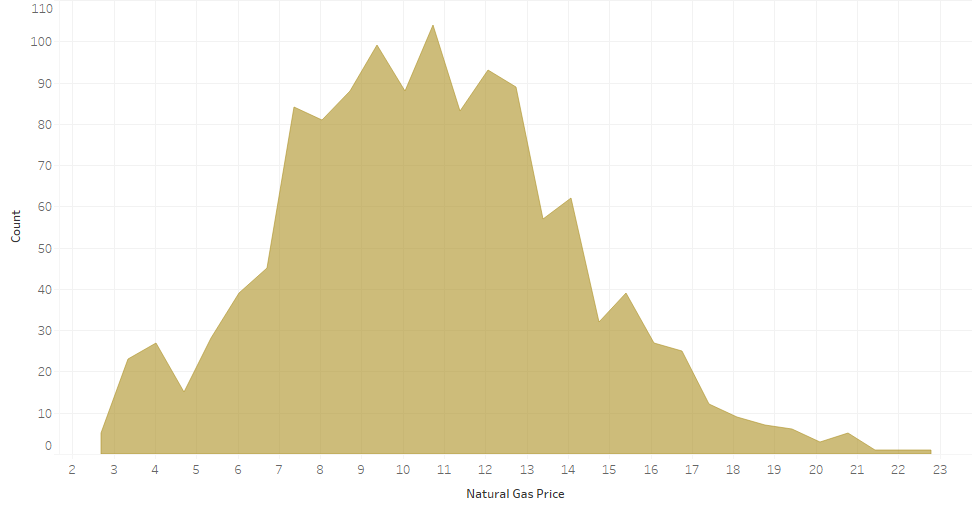
\includegraphics[width=0.7\textwidth]{Images/nGas.png}
\caption{Natural Gas Price Distribution.}
\end{center}
\end{figure}
\bigskip

The idea is to use the price of the resources from which electricity is produced to have an idea of what the price of the good could be. The choice of having the natural gas price as a variable in the data set goes in this sense. It would make sense to actually do the same for \textbf{oil}, but \textit{Eurostat} does not contain any data set with related price per country. Options could be either to use the US dollar price per barrel, which is the same for all countries or the pump price for gasoline. The choice falls on the latter, being considered as a good proxy for what is being tried to be measured. The data is available from the World Bank, and observations are recorded once every two years.\\

Electricity, as discussed in the introduction, is not only produced by burning coal, oil or natural gas, but also by using \textbf{renewable resources}. The share of electricity produced using sustainable practices on the total of electricity produced by each single country is also included in the data set. This information is recorded once a year and available from \textit{Eurostat}. However, some years are incomplete, specifically those before 2004, so those missing records are topped up with data from \textit{World Bank}. The sets from the two different sources describe the same information, e.g. for data regarding 2004, they are almost equivalent: however, just pasting data could be dangerous so normalization of the world bank information is carried out by multiplying each country value for 2000-2003 by a factor that makes records for 2004 match for both sources. \\

\noindent Another variable that takes in consideration the level of sustainability of the electricity produced is the energy \textbf{intensity}. This indicator is used to monitor progress towards United Nations' goal on climate action and on affordable and clean energy and, as anticipated in the introduction, it is calculated as the ratio between energy-related GHG emissions and gross inland consumption of energy. The data on energy emissions are being sourced from the GHG emissions reported to the UNFCCC. Information is normalized with respect to year 2000, which is used as a benchmark. This variable hence expresses how fast that particular economy is in its path towards decarbonization. Data is recorded annually and sourced from \textit{Eurostat}.\\

\noindent It is also important to consider the supply side in this context: how much each country is consuming in terms of energy. \textit{Eurostat} provides information regarding the quantity of oil equivalent (in kilograms), and this data is recorded annually. This indicator measures how much energy every citizen consumes at home excluding energy used for transportation. Since the indicator refers to final energy \textbf{consumption}, only energy used by end consumers is considered. The related consumption of the energy sector itself is excluded.\\

\noindent Many European countries do not really have the capacity to produce enough electricity in order to be self-sufficient. The \textbf{dependency} indicator shows the share of total energy needs of a country met by imports from other countries. It is calculated from energy balances as net imports divided by the gross available energy. The formula is: $$ dependence = \frac{(imports – exports)}{GAE},$$ where GAE is the Gross Available Energy. A negative value indicates net exporter: a country that exports more fuels than it consumes. In the context of of the data set at hand this happens only for \textit{Norway}. Values higher than 100 generally refer to the build of stocks (increase of fule in stocks), yet might be also a result of statistical discrepancies in raw data. This information is available from \textit{Eurostat} and recorded once a year.\\

\noindent The electricity price is also, and maybe most importantly, dependent on how wealthy that single country is. \textit{Eurostat} provides the value of the \textbf{Real Gross Domestic Product} per capita, with data being published every quarter of year. Real in this context means deflated, so leaving prices unchanged. This is key: while the Gross Domestic Product tends to increase every year (given that the country is an inflation regime), the real GDP might be decreasing if, at those prices level, on average the citizens have a lower purchasing power. The reader could wonder why to exclude the average increase in prices from the consideration, although there is a clear correlation between increase and electricity price: the higher the increase in prices the higher the expected increase in the electricity bill. The answer lies in the fact that the \textbf{inflation} variable \textit{hides} the electricity price change variable itself: the average increase in prices is computed on a basket of goods electricity is part of, so it would be too easy to actually use this our variable in our models. The dependent variable exogeneity assumption would not met.

\section*{Dynamic Model}

\chapter*{Conclusions}

\bibliography{references}{}
\bibliographystyle{plain}

\end{document}